\documentclass[a4paper,11pt]{article}
\usepackage{geometry}
\geometry{left=1in, right=1in, top=1in, bottom=1in}

% Load xcolor first with all necessary options
\usepackage[table]{xcolor}
\definecolor{mygreen}{rgb}{0.82, 0.94, 0.75}
\definecolor{mygreen2}{rgb}{0.67, 0.88, 0.69}
\definecolor{codegreen}{rgb}{0,0.94,0}
\definecolor{codegray}{rgb}{0.5,0.5,0.5}
\definecolor{codepurple}{rgb}{0.58,0,0.82}
\definecolor{backcolour}{rgb}{0.95,0.95,0.92}

\usepackage{titlesec}
\usepackage{amsmath}  % For mathematical symbols and equations
\usepackage{yhmath}
\usepackage{amssymb}%For some mathrelationsymbol
\usepackage{extarrows}
\usepackage{enumerate}
\usepackage{makecell} % 表格内换行
\usepackage{paralist}
\usepackage{datetime}
\usepackage{siunitx}
\usepackage{graphicx}  % For including figures
\graphicspath{{./figure/}}
\DeclareGraphicsExtensions{.pdf,.jpeg,.png,.jpg}
\usepackage{wrapfig}
\usepackage{bm}       % 同时黑体斜体
\usepackage{listings} % 插入代码
\usepackage[all]{xy}
\usepackage{esint}
\usepackage{bigints}
\usepackage{mathrsfs}
\usepackage{tcolorbox}
\usepackage{ulem}
\usepackage{tikz}
\usepackage{fontawesome5}
\usepackage{tasks}
\usepackage[hidelinks]{hyperref} %removing red boxes around references
\usepackage{fancyhdr} % 页眉页脚 header&footer
\usepackage{calc} % For calculating widths
\usepackage{tocloft}
\usepackage{booktabs} % For formal tables
\usepackage{longtable}
\usepackage{array}
\usepackage{multirow}
\usepackage{multicol} % Required for multicolumn within a column
\usepackage{caption}

\captionsetup[table]{
  labelfont=bf, % Makes the "Table:" label bold
}

\captionsetup[figure]{labelfont=bf}

% Custom styling for the Python code
\lstdefinestyle{mystyle}{
    backgroundcolor=\color{backcolour},   
    commentstyle=\color{codegreen},
    keywordstyle=\color{magenta},
    numberstyle=\tiny\color{codegray},
    stringstyle=\color{codepurple},
    basicstyle=\tiny, % Adjusting the code size here
    breakatwhitespace=false,         
    breaklines=true,                 
    captionpos=b,                    
    keepspaces=true,                 
    numbers=left,                    
    numbersep=5pt,                  
    showspaces=false,                
    showstringspaces=false,
    showtabs=false,                  
    tabsize=2
}
\lstset{style=mystyle}

\begin{document}

\begin{center}
\textbf {\Large REPORT SUBMISSION FORM}
\end{center}

\begin{figure}[ht]
\begin{flushright}

\includegraphics[width=0.28\textwidth]{USMlogo}
\end{flushright}
\end{figure}

\large
\begin{tabular}{lcl}
Name & : &\dotuline{TAN WEi LIANG\hfill}\\
\\
Partner's Name &: &\dotuline{AINA IMANINA BINTI MOHB KHOZIKIN\hfill}\\
\\
Group& : &\dotuline{M5B\hfill}\\
\\
Experiment Code& :&\dotuline{1OS3\hfill}\\
\\
Experiment Title&: &\dotuline{Geometric Optics\hfill}\\
\\
Lecturer’s/Examiner’s&: &\dotuline{DR. John Soo Yue Han\hfill}\\ 
Name\\
\\
Starting Date &: &\dotuline{15/04/2024\hfill}\\
(1st session)\\
\\
Ending Date &: &\dotuline{22/04/2024\hfill}\\
(2nd session)\\
\\
Submission Date &: &\dotuline{29/04/2024\hfill}\\
\\
\end{tabular}


\newpage
\begin{center}
\textbf{\Large DECLARATION OF ORIGINALITY}
\end{center}
\bigskip
I, \textbf{TAN WEI LIANG 22302889}
hereby declare that this laboratory report is my own work. I further declare that:

\begin{enumerate}
    \item The references/bibliography reflect the sources I have consulted, and
    \item I also certify that this report has not previously been submitted for assessment in this or any other units, and that I have not copied in part or whole or otherwise plagiarized the work of other students and/or persons.
    \item Sections with no source referrals are my own ideas, arguments, and/or conclusions.\\\\
\end{enumerate}

\noindent Signature: \hrulefill \hfill Date: \uline{28/04/2024}

\newpage
\begin{center}
\vspace*{1cm}
\textbf{\Large GEOMETRIC OPTICS}

\vspace{3.0cm}
\textbf{By}\\

\vspace{3.0cm}
\textbf{TAN WEI LIANG} \\

\vspace{3.0cm}
\textbf{April 2024}\\

\vfill
\textbf{\large First Year Laboratory Report}
\end{center}


\newpage
\phantomsection
\section*{\large \center GEOMETRIC OPTICS}
\addcontentsline{toc}{section}{ABSTRACT}
\section*{\large \center ABSTRACT}
\label{sec:ABSTRACT}
The title of this experiment is GEOMETRIC OPTIC. In this experiment, focusing on the relationships between focal length, object distance, and image distance, along with the study of magnification across various setups. Through the use of both converging and diverging lenses, the experiment investigated how light manipulation varies with changes in lens type and configuration. Experimental results confirmed the focal length of the converging lens to be \( \bar{f} = (10.04 \pm 0.04) \, \text{cm} \). The diverging lens produced a virtual image positioned at (\(-7.5\pm 0.1\)) cm, exhibiting properties such as being upright and reduced image which further than the object to the lens. The magnification of the virtual image is 0.375, indicated the virtual image is upright. Additionally, the magnification values for the telescope and microscope were 1.78 and -17.82.
\newpage 
\phantomsection
\section*{\large \center ACKNOWLEDGEMENTS}
\addcontentsline{toc}{section}{ACKNOWLEDGEMENTS}
\label{sec:ACKNOWLEDGEMENTS}
\quad First and foremost, I express my sincere appreciation to DR. John Soo Yue Han, our distinguished lecturer and examiner, for the invaluable guidance and unwavering support extended throughout our scientific exploration. I extend my sincere gratitude to my experiment partner, Aina Imanina Binti Mohb Khozikin. Her invaluable cooperation and dedication throughout both experiments were instrumental to the success of this project. I appreciate her commitment, expertise, and teamwork, which made these scientific endeavours both productive and enjoyable. A heartfelt acknowledgment is also extended to Dr. John Soo Yue Han for his dedicated efforts in creating the manual in 2020, elevating its clarity and educational significance. This collective endeavor has significantly enhanced our scientific learning journey, and I extend genuine gratitude to everyone mentioned for their noteworthy contributions.

\newpage
\renewcommand{\contentsname}{\centering CONTENTS}
\renewcommand{\cftsecleader}{\cftdotfill{\cftdotsep}} % Ensures dotted lines for sections
% Adjust the dot separation
\renewcommand{\cftdotsep}{1.0} % Default is 4.5, decrease for more dots
\tableofcontents
\phantomsection
\addcontentsline{toc}{section}{CONTENTS}
\label{sec:CONTENTS}

\newpage
\phantomsection
\addcontentsline{toc}{section}{LIST OF TABLES}
\label{sec:LIST OF TABLES}
\listoftables

\newpage
\phantomsection
\addcontentsline{toc}{section}{LIST OF FIGURES}
\label{sec:LIST OF FIGURES}
\listoffigures

\newpage
\phantomsection
\section*{\center INTRODUCTION}
\addcontentsline{toc}{section}{INTRODUCTION}
\label{sec:INTRODUCTION}
\quad 
The study of light and its interaction with various media is fundamental to optical physics. Geometric optics, in particular, offers a simplified perspective by treating light as straight-line rays and analyzing its behavior through refraction and reflection. This experiment focuses on the practical exploration of these principles using thin lenses to manipulate light and form images, which is crucial in optical devices like telescopes, and microscopes. By employing both convex and concave lenses, we examine the thin lens equation and magnification formulas in a controlled setting. The experiment not only aims to measure the focal lengths and magnification provided by these lenses but also to demonstrate how lenses can be combined to telescopes and microscopes using lens systems. In telescopes, two lenses are arranged to allow the observation of distant objects by magnifying the image produced by the objective lens with an eyepiece. Similarly, the microscope setup uses a sequence of lenses to greatly enhance the image of very small, close objects, highlighting how the focal properties and placement of each lens can achieve high magnification levels.
%%%%%%%%%%%%%%%%%%%%%%%%%%%%%%%%%%%%%%%%%
% Theory Part
\newpage
\phantomsection
\section*{\center THEORY}
\addcontentsline{toc}{section}{THEORY}
\label{sec:THEORY}
\subsection*{Basic Geometrical Optics}

A lens is defined to be thin if its thickness is small compared to the other distances involved. For a thin lens,

\begin{equation}
\frac{1}{f} = \frac{1}{o} + \frac{1}{i},
\end{equation}

where \(f\) is the focal length, \(o\) the distance between the object and the lens, and \(i\) the distance between the image and the lens. This equation is known as the thin lens equation. By measuring \(o\) and \(i\), the focal length can be determined. Recall that if the image is on the opposite side of the lens with respect to the object, \(i\) will be positive, and the image is real; if the image is on the same side instead, \(i\) will be negative, and the image is virtual.\\

A virtual image cannot be viewed on a screen; it forms where the backwards extensions of diverging rays cross. You can see a virtual image by looking at it through a lens or mirror. Like all images, a virtual image formed by a lens or mirror can serve as the object of another lens or mirror.\\

The image formed by a thin lens can be described by its orientation (upright or inverted) and by its magnification (enlarged or reduced compared to the original object). Magnification (\(M\)) is the ratio of image size (\(s_i\)) to object size (\(s_o\)). It can also be measured using the ratio between the image and object distances as follows:

\begin{equation}
|M| = \frac{s_i}{s_o}, \quad M = -\frac{i}{o}.
\end{equation}

Note that if the image is upright, \(M\) is positive; if the image is inverted, \(M\) is negative.
\begin{figure}[htbp]
\centering
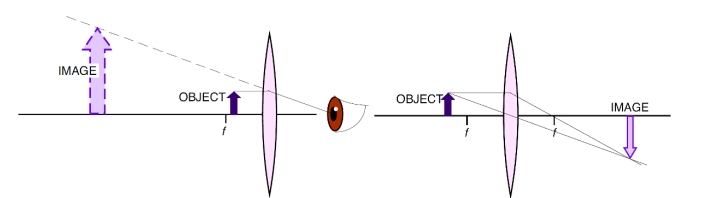
\includegraphics[width=0.8\linewidth]{G1}
\caption{Positions of images when placed closer (left) / further (right) to a convex lens.}
\label{6}
\end{figure}
In this experiment, two kinds of lenses are used: the convex lens (also known as positive / convergent lens) which has a positive focal length, and the concave lens (negative / divergent lens) which has a negative focal length. When an object is placed closer to a convex lens than its focal length, the lens works as a magnifier and produces an enlarged virtual image; when an object is placed further from it than its focal length, the lens produces an inverted, real image, and it could be reduced or enlarged, depending how close the object is to the focal point(\textbf{Figure 1}).\\

When two thin lenses are used, we can analyse the distances by taking the image from one lens as the object for the second. The observer views an image that is ``an image of an image''. The overall magnification $M$ of a two-lens system is equal to the product of the magnifications of the individual lenses, $M_1$ and $M_2$:

\begin{equation}
M = M_1M_2 = \left(-\frac{i_1}{o_1}\right) \left(-\frac{i_2}{o_2}\right),
\end{equation}

where $(o_1, i_1)$ and $(o_2, i_2)$ are the object-image distance pairs for each lens system.

\subsection*{Telescopes and Microscopes}

The telescope and the microscope are two important optical devices that use two lenses. In each device a primary lens (the objective) forms a real image and a secondary lens (the eyepiece) is used as a magnifier to make an enlarged virtual image.\\

An astronomical refractor telescope is used to view large objects that are at large distances from the lenses. Firstly, the objective lens produces a first real image of a very far away object (\(o \rightarrow \infty\)). So using the thin lens equation, we have

\begin{equation}
\frac{1}{f} = \frac{1}{\infty} + \frac{1}{i} \approx \frac{1}{i},
\end{equation}

where the image forms coincident with the objective’s focal point (\(f_o\)). The eyepiece is then placed close to that first image, so that the image formed by the objective lens falls within the eyepiece’s focal length (\(f_e\)) and is thus magnified. The closer the first image is to the eyepiece’s focal point, the longer the distance to the final image.

\begin{figure}[htbp]
\centering
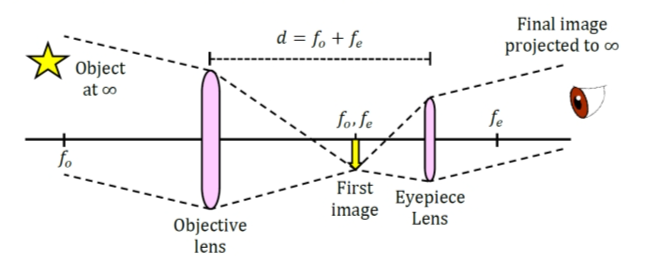
\includegraphics[width=0.7\linewidth]{G2}
\caption{Principles of the refractor telescope. The objective lens forms the first image, then the eyepiece lens greatly magnifies the first image.}
\label{6}
\end{figure}

Astronomical telescopes are usually built so that the first image forms exactly at the focal point of the eyepiece lens. In this case, the separation between the lenses is exactly $d = f_o + f_e$, which is the length of the telescope tube. The magnification of an astronomical telescope with the object at infinity, and with $f_o$ and $f_e$ both coincident with the first image, is defined as the ratio of the focal length of the objective to that of the eyepiece:

\begin{equation}
M = \frac{f_o}{f_e} = \frac{i_o}{o_e}.
\end{equation}

Note that this equation is only valid for a telescope with $d = f_o + f_e$.
\newpage
\begin{figure}[h]
\centering
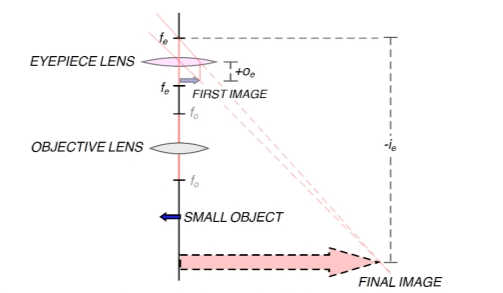
\includegraphics[width=0.6\linewidth]{G3}
\caption{Principles of the microscope. The objective lens forms the first image, this image is real, inverted, and reduced. The eyepiece lens forms the final image using the first image as its object, this final image is virtual and greatly enlarged.}
\label{6}
\end{figure}

A compound microscope is used to view small objects that are very close to the lenses. A microscope is useful when the magnification required is more than what can be obtained with a single magnifier lens. Firstly, the objective lens produces a first real image of the object, by having the object be just beyond its focal length. The eyepiece will then be placed very close to that first image, so that the first image falls within the eyepiece's focal length and is thus greatly enlarged.

\subsection*{LINEST function}
LINEST function is a function that calculates the statistics for a line that best fits your data. It uses the "least squares" method to find the slope and intercept of the line, and returns an array that describes the line. The function also returns the F statistic, which measures how well the line fits the data.\\
\newpage
\phantomsection
\section*{\center EXPERIMENTAL METHODOLOGY}
\addcontentsline{toc}{section}{EXPERIMENTAL METHODOLOGY}
\label{sec:EXPERIMENTAL METHODOLOGY}
% Content for the EXPERIMENTAL METHODOLOGY section goes here.
\begin{figure}[htbp]
\centering
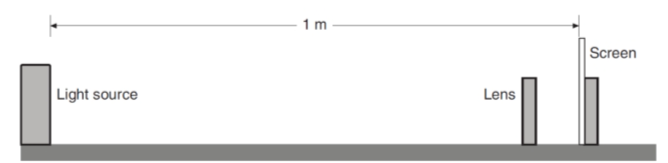
\includegraphics[width=0.7\linewidth]{GM1}
\caption{experimental setup for Part A}
\label{6}
\end{figure}
% Part A
The experiment of \textbf{Part A} initiates by positioning the light source and the screen at the 0 cm and 100 cm marks on the optics bench, respectively, ensuring that the crossed-arrow object on the light source is facing the screen. The $+10$ cm lens is initially placed close to the screen, then gradually moved away until a clear image of the crossed-arrow object is formed on the screen. The position of the lens, along with the sizes of the object ($s_o$) and its image on the screen ($s_i$), are meticulously recorded. The lens is then shifted, without moving the positions of the screen or light source, to a second location where a focused image is again observable with the partial crossed-arrow pattern on the screen, the image and object sizes are measured as the distance between two index marks on the pattern.\\

The experiment is repeated by adjusting the screen position to 90 cm, 80 cm, 70 cm, 60 cm, and 50 cm, respectively. At each stage, two lens positions that yield clear images are found, without the necessity of measuring object and image sizes.\\

For the analysis phase, the first step involves calculating the object distance ($o$) as the distance between the lens and the light source, and the image distance ($i$) as the distance between the lens and the screen for each lens position. Subsequently, the reciprocal of these distances, $\frac{1}{o}$ and $\frac{1}{i}$, are computed. These reciprocal values are plotted on a graph of $\frac{1}{i}$ versus $\frac{1}{o}$ to derive a linear best-fit line, from which the $x$- and $y$-intercepts are determined. The focal length ($f$) of the lens is then calculated from each intercept, and the percentage difference between these focal lengths is evaluated to ascertain the precision of the experiment. The mean of the two focal lengths provides a final value for $f$.\\

Additionally, for the initial two sets of measurements, the magnification ($M_d$) is calculated using the object and image distances, while the absolute magnification ($\lvert M_s \rvert$) is determined from the object and image sizes. The average of the absolute values of magnification obtained from both methods is recorded, and the percentage difference between these values is calculated to assess the consistency between the two magnification measurements.\\

\newpage
% Part B
\begin{figure}[htbp]
\centering
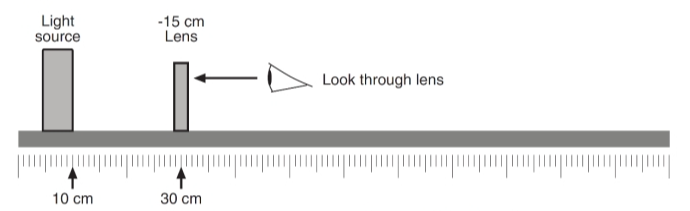
\includegraphics[width=0.7\linewidth]{GM3}
\caption{experimental first setup for Part B}
\label{6}
\end{figure}
The experiment of \textbf{Part B} commenced by placing a diverging lens with a focal length of $-15$ cm on an optical bench at the $30$ cm mark. Subsequently, a light source equipped with a crossed-arrow object was positioned at the $10$ cm mark on the same bench, directed towards the lens. Observations were then made by looking through the lens towards the light source. This setup allowed for the assessment of the image characteristics such as orientation (upright or inverted), size (enlarged or reduced), and relative position (closer to or further from the lens than the object).\\

\begin{figure}[htbp]
\centering
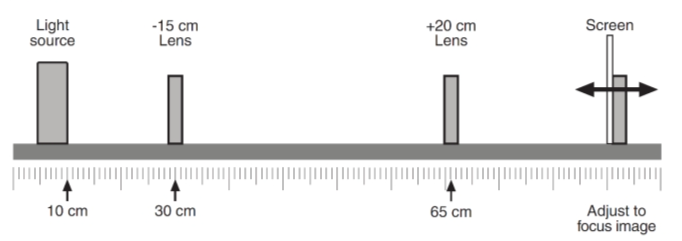
\includegraphics[width=0.7\linewidth]{GM4}
\caption{experimental second setup for Part B}
\label{6}
\end{figure}
Following the initial observations, a converging lens with a focal length of $+20$ cm was placed at the $65$ cm mark on the optical bench. A viewing screen is placed behind this lens and is moved until a clear image of the virtual image is visible on the screen. \\

\begin{figure}[htbp]
\centering
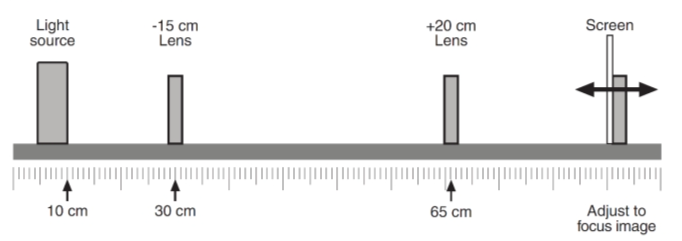
\includegraphics[width=0.7\linewidth]{GM4}
\caption{experimental third setup for Part B}
\label{6}
\end{figure}
To further investigate the lens system, the negative lens is removed, causing the image on the viewing screen to go out of focus. The light source is then adjusted to a new position where a clear image is refocused on the screen without moving the converging lens or the viewing screen. This final position of the light source is recorded.\\

The distances between the initial light source position and the diverging lens (object distance $o$), as well as between the diverging lens and the virtual image (image distance ($i$), a negative value), were calculated which it is a negative value. Magnification factor ($M$) of the virtual image is calculated, and state whether it is upright / inverted.\\

For a comprehensive understanding, a scaled diagram was drafted to show the positions of the light source (initial), both lenses, the screen, and both the real and virtual images. Arrows ($\uparrow$) were used to represent the objects and images, varying in height and direction to reflect their magnification characteristics accurately.\\

% Part C
\begin{figure}[htbp]
\centering
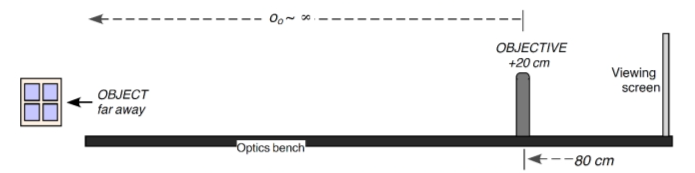
\includegraphics[width=0.7\linewidth]{GM6}
\caption{experimental setup for Part C}
\label{6}
\end{figure}
The experiment of \textbf{Part C} initiates by an optics bench was aligned such that its \(0 \, \text{cm}\) mark faced an open window to ensure natural light could be utilized. A converging lens with a focal length of \(+20 \, \text{cm}\) was positioned at the \(80 \, \text{cm}\) mark on the bench, and a viewing screen was placed at the opposite end. The experiment commenced by gradually moving the viewing screen towards the lens until a distinct image of an external object was produced, with the position of the sharpest image captured and recorded, including the nature of the image in terms of orientation, size, and reality. Subsequently, a \(+10 \, \text{cm}\) lens, acting as an eyepiece, was placed approximately \(10 \, \text{cm}\) behind the first image, forming a rudimentary telescope with an estimated length of \(30 \, \text{cm}\). The viewing screen was then removed, and the eyepiece was manually adjusted while observing with a single eye until a clear , magnified image was achieved, with the final eyepiece position also recorded.\\

These measurements allowed for the subsequent analysis of distances between the objective lens and the first image ($i_o$), between the first image and the eyepiece ($i_e$), and from the eyepiece to the final image ($i_e$), enabling the calculation of the magnification of the second image ($M_e$) and the total magnification of the telescope setup ($M$). Additionally, a theoretical magnification ($M_{theo}$) was deduced using the known values of the focal lengths of the objective ($f_o$) and eyepiece ($f_e$), and a comparison was made with the experimental magnification to assess the percentage discrepancy.
%%%%%%%%%%%%%%%%%%%%%%%%%%%
% Part D
\begin{figure}[htbp]
\centering
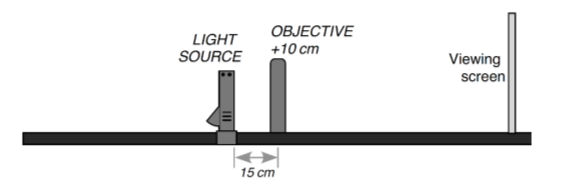
\includegraphics[width=0.7\linewidth]{GM7}
\caption{experimental setup for Part D}
\label{6}
\end{figure}

The experimental of \textbf{Part D} setup was initiated by positioning a +10 cm converging lens at a 60 cm mark on an optical bench. A light source was then installed at the 45 cm mark, projecting an image of crossed arrows towards the lens. Opposite the light source and lens, a viewing screen was placed to capture the image. The screen was gradually moved closer to the lens until a sharp image of the arrows was formed, with the image's characteristics such as location of image, orientation, size and reality being meticulously recorded.\\

Subsequently, a +20 cm lens was mounted directly behind the initial viewing screen. This lens served as the objective lens of our microscope. We closely observed the lens, adjusting our position to achieve a clear and enlarged image of the back of the viewing screen, which was rendered sharp by the arrangement of the optical elements. Upon removal of the viewing screen and the light source, we hold a copy of the grid to the former position of the screen using a rubber band, replicating the original setup of the light source. This grid, containing a small message at its center, acted as the new object of interest. The screen, now holding the grid, was placed back at the light source's previous location. By peering through the eyepiece lens, we sought out the small message on the grid, adjusting the lens slightly for a focused image and recorded the eyepiece's final position.\\

The gathered data, including various distances between the light source, objective lens, screen, and eyepiece, were used to compute specific distances such as object distance (\( o_o \)), image distance (\( i_o \)), and the distance from the back of the screen to the eyepiece lens (\( o_e \)). We then calculated the distance from the eyepiece to the final image (\( i_e \)). These distances allowed us to determine the magnification produced by each lens, denoted (\( M_o \) for the objective and (\( M_e \)) for the eyepiece, as well as the total magnification (\( M \)) of the system.\\
%%%%%%%%%%%%%%%%%%%%%%%%%%%%%%%%%%%%%%%%%%
\newpage
\phantomsection
\section*{\center DATA ANALYSIS}
\addcontentsline{toc}{section}{DATA ANALYSIS}
\label{sec:DATA ANALYSIS}
% Content for the DATA ANALYSIS section goes here.
\textbf{All calculation of the experments are attached in the Appendices.}\\
\\
\textbf{PART A}\\
\\
The data collected from the experiment in \textbf{Part A} is summarized in \textbf{Table 1}.
\begin{table}[ht]
\centering
\caption{Experimental data for Part A}
\resizebox{\textwidth}{!}{ % Resize table to fit the width of the page
\begin{tabular}{|c|c|c|c|c|c|c|c|c|}
\hline
\multicolumn{2}{|c|}{\multirow{2}{*}{\textbf{Positions} (\(\pm\)0.1 cm)}} &&&&&&\\ 
\multicolumn{2}{|c|}{} & {\(o\) (\(\pm\)0.1cm)} & \(i\) (\(\pm\)0.1cm) & \textbf{\(1/o\)} & \textbf{\(1/i\)} &  \(s_o\) (\(\pm\)1mm) & \(s_i\) (\(\pm\)1mm) \\ \cline{1-2}
\textbf{Screen} & \textbf{Lens} &  & & & & &\\ 
\hline
\multirow{2}{*}{100.0} & 88.8 & 88.8 & 11.2 & 0.0113 & 0.0893 & 40 & 5 \\\cline{2-8}
                       & 11.1 & 11.1 & 88.9 &  0.0901 & 0.0112 & 5 & 35\\ \cline{1-8}

\multirow{2}{*}{90.0}  & 78.5 & 78.5 & 11.5 &  0.0127 & 0.0870\\ \cline{2-6}
                       & 11.6 & 11.6 & 78.4 &  0.0862 & 0.0128\\ \cline{1-6}
                       
\multirow{2}{*}{80.0}  & 68.3 & 68.3 & 11.7 &  0.0146 & 0.0855\\ \cline{2-6}
                       & 11.7 & 11.7 & 68.3 &  0.0855 & 0.0146\\ \cline{1-6}

\multirow{2}{*}{70.0}  & 57.8 & 57.8 & 12.2 &  0.0173 & 0.0820 \\ \cline{2-6}
                       & 12.0 & 12.0 & 58.0 & 0.0833 & 0.0172\\ \cline{1-6}

\multirow{2}{*}{60.0}  & 46.9 & 46.9 & 13.1 & 0.0213 & 0.0763  \\ \cline{2-6}
                       & 12.8 & 12.8 & 47.2 & 0.0781 & 0.0212\\ \cline{1-6}

\multirow{2}{*}{50.0}  & 35.9 & 35.9 & 14.1 &  0.0279 & 0.0709 \\ \cline{2-6}
                       & 14.0 & 14.0 & 36.0 &  0.0714 & 0.0278  \\ \cline{1-6}
\end{tabular}
}
\label{tab:experimental_data}
\end{table}
\\
The result after LINEST function in Excel is summarized in \textbf{Table 2}.
\begin{table}[h!]
\centering
\caption{LINEST() results}
\begin{tabular}{|c|c|c|c|}
\hline
m & -0.992 & 0.0992 & c  \\ 
\hline
\textbf{$\sigma_m$} & 0.009 & 0.0005 &\textbf{$\sigma_c$}\\ 
\hline
\textbf{$r^2$} & 0.9992 & 0.0010 &\textbf{$\sigma_y$}\\ 
\hline
\end{tabular}
\end{table}
\\
From the data obtained above, we see that every graph has a correlation coefficient of 0.9992. This shows that there is quite strong positive correlation between the variables, and the equation is well verified. \\
\\
By using LINEST, we found that:
\begin{itemize}
  \item[] gradient of the graph, $m = (-0.992 \pm 0.009)$
  \item[] Y-intercept of the graph, $c = (0.0992 \pm 0.0005)\, \text{cm}^{-1}$\\
\end{itemize}
The result of focal length of lens is summarized in \textbf{Table 3}.
\begin{table}[ht]
\centering
\renewcommand{\arraystretch}{1.1}
\caption{Focal length of the lens}
\begin{tabular}{|c|c|c|c|c|c|c|c|}
\hline
\textbf{x-intercept} & 0.1000 &\textbf{\( f_x \)} & 10.00 & \(\pm\) &0.01 & cm \\
\hline
\textbf{y-intercept} & 0.0992 &\textbf{\( f_y \)} & 10.08 & \(\pm\) &0.04 & cm \\
\hline
\multicolumn{1}{c}{}& \multicolumn{1}{c|}{}& \( \bar{f} \) & 10.04 & \(\pm\) &0.04  & cm \\
\cline{3-7}
\multicolumn{1}{c}{}& \multicolumn{1}{c|}{}&\textbf{\% diff.} &0.40 &\multicolumn{3}{c|}{ \%} \\
\cline{3-7}
\end{tabular}
\label{your-label}
\end{table}
\newpage
\noindent The result of magnification of lens is summarized in \textbf{Table 4}.
\begin{table}[h!]
\centering
\caption{Magnification of lens}
\begin{tabular}{|c|c|c|c|c|}
\hline
\textbf{Using \( o \) and \( i \):} & \( M_{d,1} \)& 0.126 & \( M_{d,2} \)& 8.009 \\
\hline 
\textbf{Using \( s_o \) and \( s_i \):} & \( |M_{s,1}| \) & 0.125 & \( |M_{s,2}| \) & 7.000 \\
\hline
\multicolumn{1}{c|}{}&  \textbf{\( |M_1| \)} & 0.126 & \textbf{\( |M_2| \)} &7.505 \\
\cline{2-5}
\multicolumn{1}{c|}{}&  \textbf{\% diff.} & 0.80 \% & \textbf{\% diff.} &13.45 \% \\
\cline{2-5}
\end{tabular}
\label{tab:my_label}
\end{table}
\\
\begin{figure}[h!]
\centering
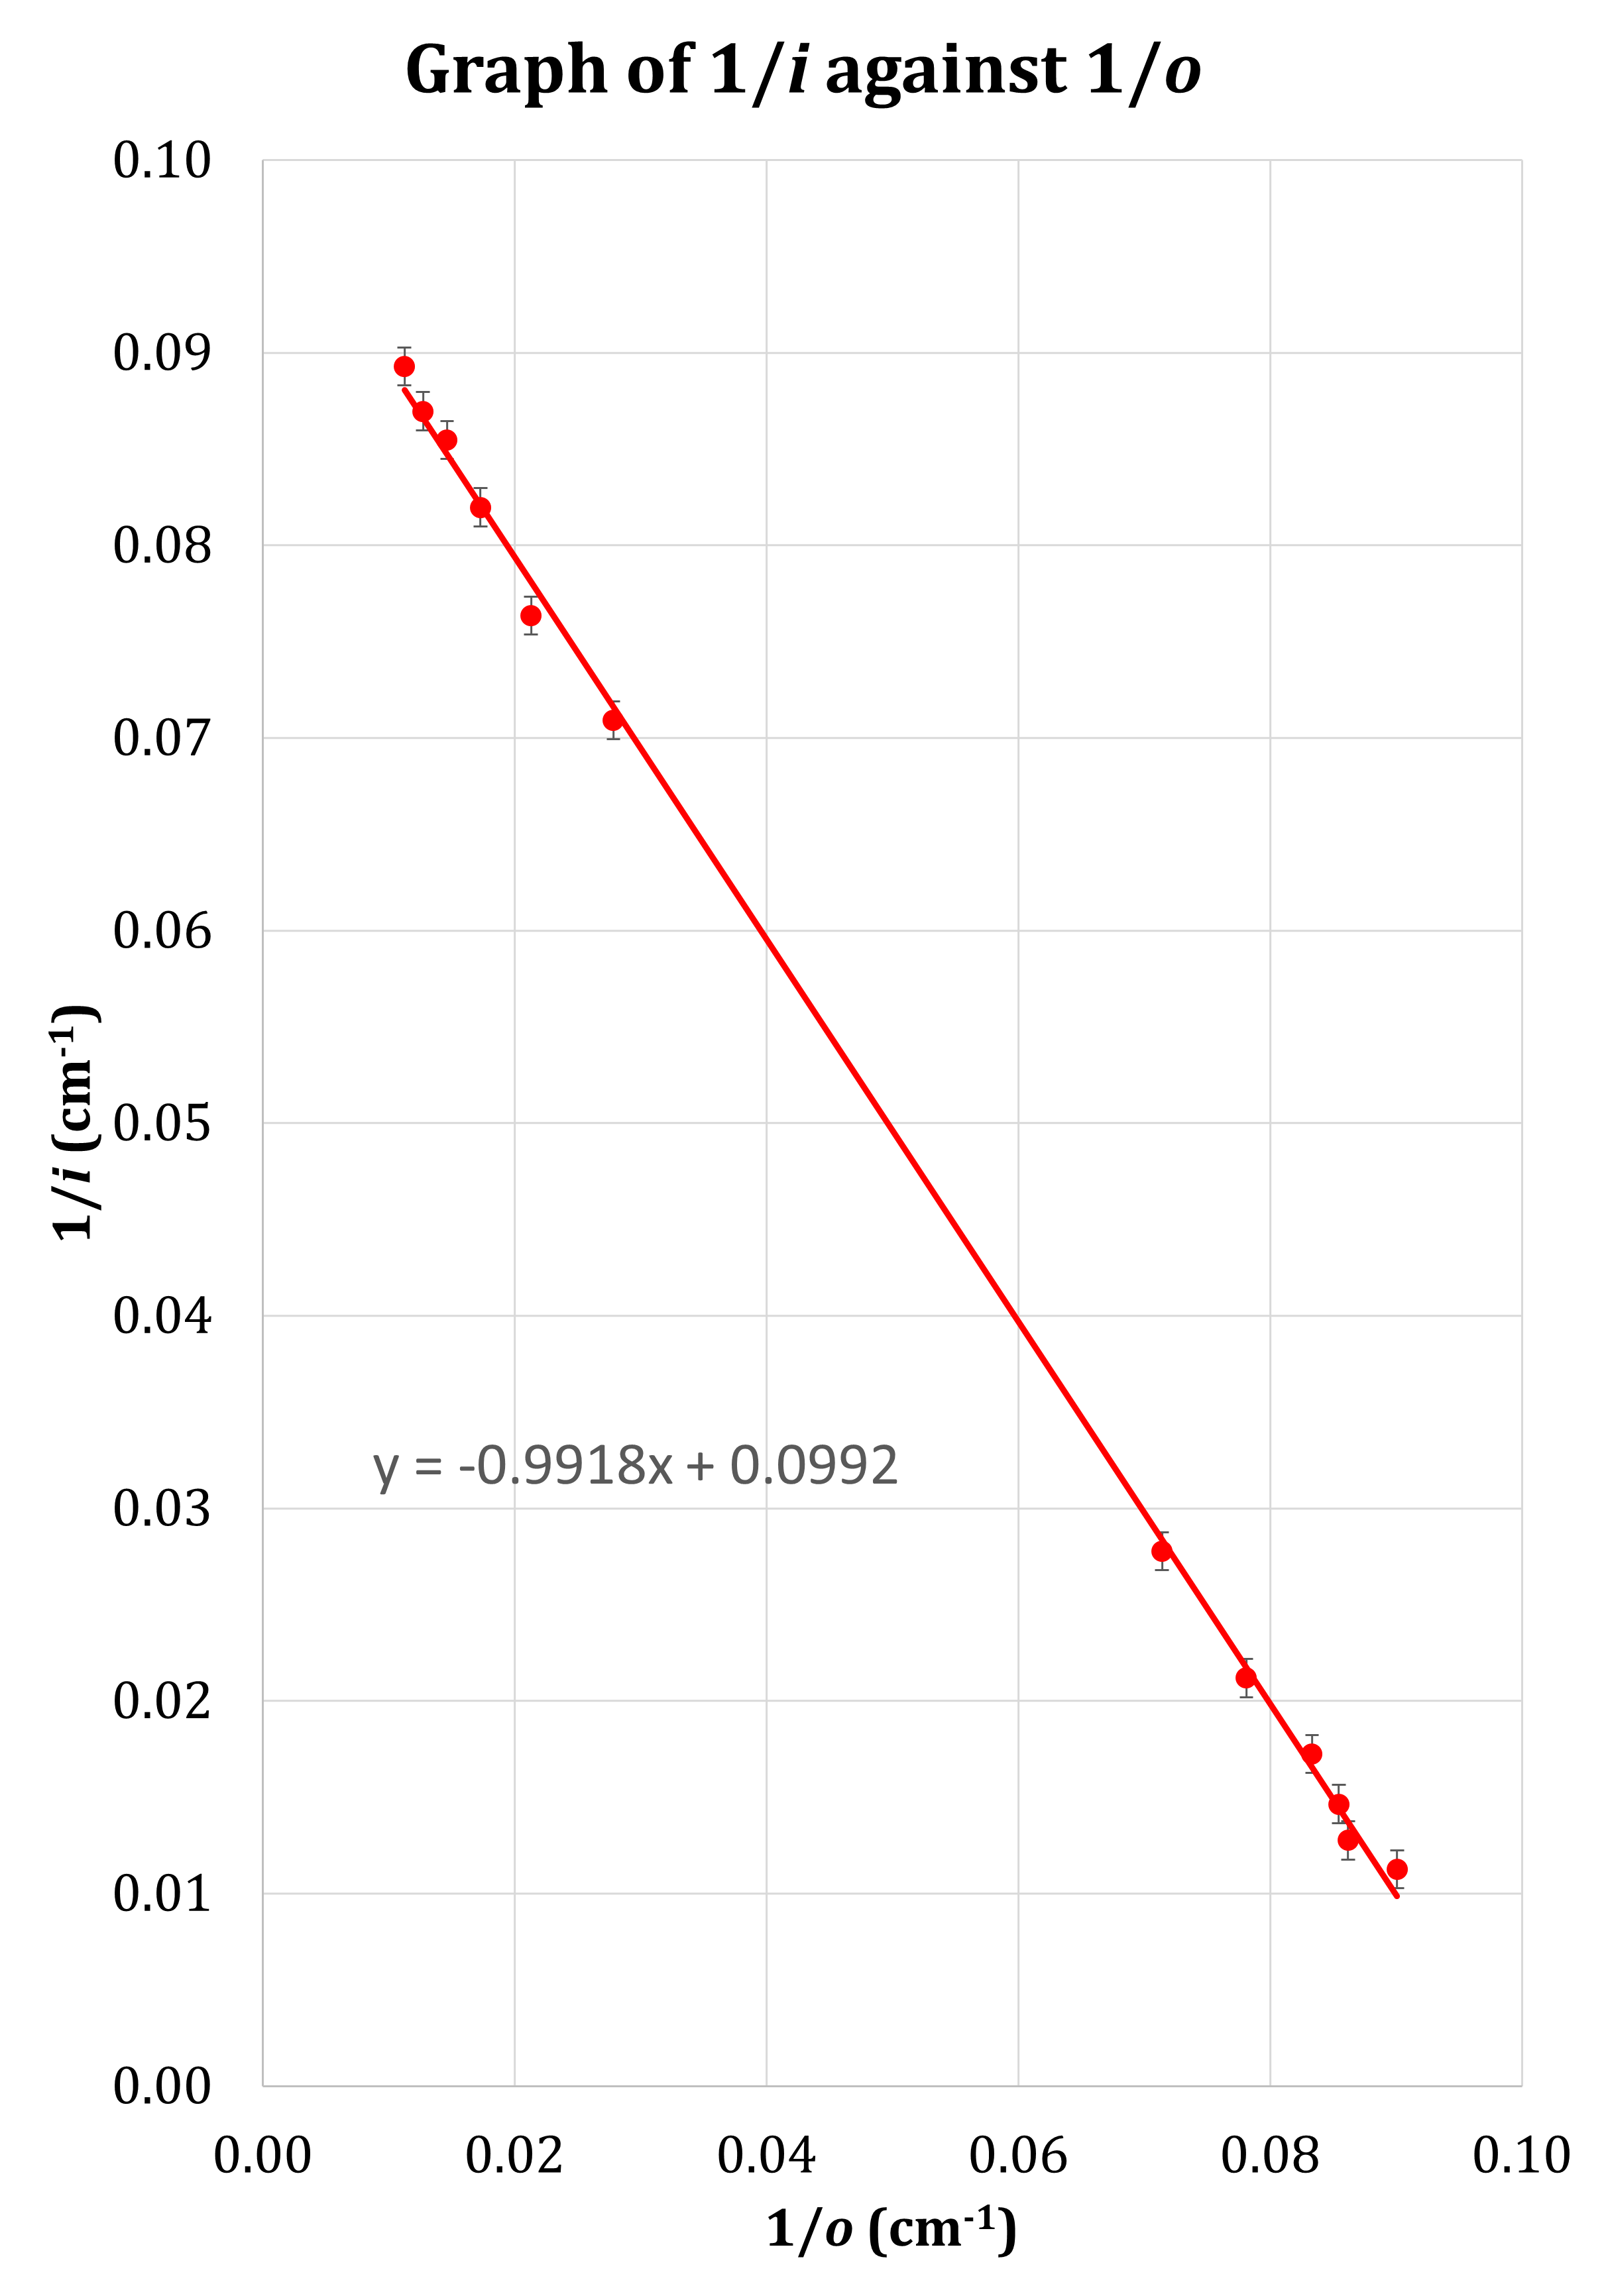
\includegraphics[width=0.8\linewidth]{GG1}
\caption{Graph of 1/i against 1/0}
\label{6}
\end{figure}

\newpage
%%%%%%%%%%%%%%%%%%%%%%%%%%%%%%%%%%%%%%%%%%
%Part B
\noindent\textbf{PART B}\\
\\
The data collected from the experiment in \textbf{Part B} is calculated and summarized in \textbf{Table 5}.
\\
\begin{table}[h!]
\centering
\caption{Experimental data for Part B}
\label{your-label}
\resizebox{\textwidth}{!}{%
\begin{tabular}{|c|c|c|c|c|c|c|c|}
\hline
\multicolumn{5}{|c|}{\textbf{Positions (\(\pm\) 0.1 cm)}} &  &  & \\
\cline{1-5}
\textbf{Light source (initial)} & \textbf{-15 cm lens} & \textbf{+20 cm lens} & \textbf{Screen} & \textbf{Light source (final)} & \(o\)(\(\pm\) 0.1 cm) & \(i\)(\(\pm\) 0.1 cm) & \textbf{\(M\)} \\
\hline
10.0 & 30.0 & 65.0 & 100.0 & 22.5 & 20.0 & -7.5 & 0.375 \\
\hline
\end{tabular}
} % Ending resizebox
\end{table}
\\
\noindent Image properties: upright, reduced, further than the object to the lens\\		
\\
The magnification, \(M\) of the virtual image is positive value indicated the virtual image is upright.
\\
\begin{figure}[htbp]
\centering
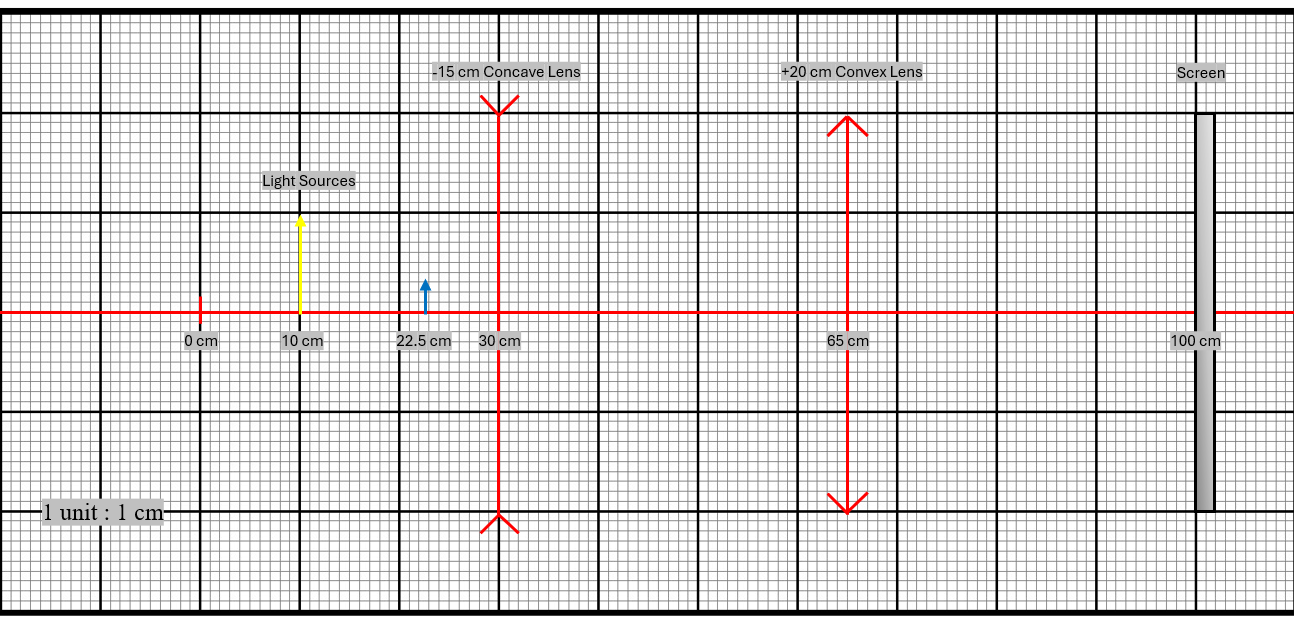
\includegraphics[width=0.999\linewidth]{GSD1}
\caption{Scaled Diagram of experiment}
\label{6}
\end{figure}
\\
%%%%%%%%%%%%%%%%%%%%%%%%%%%%%%%%%%%%%%%%%
%Part C
\textbf{PART C}
\\
The data collected from the experiment in \textbf{Part C} is calculated and summarized in \textbf{Table 6}.
\begin{table}[htbp]
\centering
\caption{Experimental data for Part C}
\label{your-label}
\resizebox{\textwidth}{!}{%
\begin{tabular}{|c|c|c|c|c|c|c|c|c|c|}
\hline
\multicolumn{3}{|c|}{\textbf{Positions} (\(\pm\) 0.1 cm)} &\(i_o\) &\(o_e\)  &\(i_e\) &\(M_e\) & \(M\) &\(M_{theo}\)  & \textbf{\% disc.} \\
\cline{1-3}
\textbf{Objective lens} & \textbf{Screen} & \textbf{Eyepiece} & (\(\pm\) 0.1 cm) &(\(\pm\) 0.1 cm) & (\(\pm\) 0.1 cm) &  & & &\\
\hline
80.0 & 98.3 & 108.6 & 18.3 & 10.3 & 343.3 & -33.33 & 1.78 & 2.00 & 11.00\\
\hline
\end{tabular}
} % Ending resizebox
\end{table}
\\
\noindent Image properties: inverted, reduced, real\\	
\\		
%%%%%%%%%%%%%%%%%%%%%%%%%%%%%%%%%%%%%%%%%
%Part D
\newpage
\noindent\textbf{PART D}
\\
The data collected from the experiment in \textbf{Part D} is calculated and summarized in \textbf{Table 7}.
\\
\begin{table}[h!]
\centering
\caption{Experimental data for Part D}
\label{your-label}
\resizebox{\textwidth}{!}{%
\begin{tabular}{|c|c|c|c|c|c|c|c|c|c|c|}
\hline
\multicolumn{4}{|c|}{\textbf{Positions (\(\pm\) 0.1 cm)}} &\(o_o\) &\(i_o\)  &\(o_e\) &\(i_e\) & \(M_o\) &\(M_e\)  & M \\
\cline{1-4}
Light source & Objective lens & Screen & Eyepiece & (\(\pm\) 0.1 cm) &(\(\pm\) 0.1 cm) & (\(\pm\) 0.1 cm) & (\(\pm\) 0.1 cm)  & (\(\pm\) 0.1 cm) &(\(\pm\) 0.1 cm) & (\(\pm\) 0.1 cm) \\
\hline
45.0 & 60.0 & 89.4 & 107.2 & 15.0 &29.4 & 17.8 & -161.8 & -1.96 & 9.09 & -17.82\\
\hline
\end{tabular}
} % Ending resizebox
\end{table}
\\
\noindent Image properties: inverted, enlarged, real\\		
%%%%%%%%%%%%%%%%%%%%%%%%%%%%%%%%%%%%%%%%%%
\newpage
\phantomsection
\section*{\center DISCUSSION}
\addcontentsline{toc}{section}{DISCUSSION}
\label{sec:DISCUSSION}
% Content for the DISCUSSION section goes here.
\qquad 
The errors for the measurements taken for a multi-variable function \(f(x,y,z,\ldots)\) where the variables \(x,y,z,\ldots\) and their uncertainties \(\delta x, \delta y, \delta z, \ldots\) are random and independent from one another, we can use the formula
of propagation of errors  to calculate the uncertainty

\begin{equation*}
\delta f = \sqrt{
\left( \frac{\partial f}{\partial x} \delta x \right)^2 +
\left( \frac{\partial f}{\partial y} \delta y \right)^2 +
\left( \frac{\partial f}{\partial z} \delta z \right)^2 +
\ldots
}
\end{equation*}
This is known as the equation for propagation of errors since we propagate the errors of \(x,y,z,\ldots\) into the derived quantity \(f\). Using these equation, we calculated the errors in Part A for \(\bar{f}\).\\

In Part A of the experiment, we determined the average focal length to be \( \bar{f} = (10.04 \pm 0.04) \) cm, which deviates by 0.40\% from the expected focal length of 10 cm. This slight discrepancy confirms the accurancy between experimental and theoretical values, indicating that our measurements closely align with theoretical expectations. The experiment produced two distinct image positions, corresponding to real and virtual images formed by a convex lens. When the object is beyond the lens's focal point, a real image is formed, while a virtual image appears when the object is between the lens and the focal point. Our results suggest that the lens behaves as if it has dual focal points, as evidenced by the calculated \( f_x = (10.00 \pm 0.01) \) cm and \( f_y = (10.08 \pm 0.04) \) cm from the x-intercept and y-intercept, respectively. Magnification values for lens positions \( s_o \) and \( s_i \) were 0.126 and 8.009, with absolute magnifications of 0.125 and 7.000, leading to mean magnification values of 0.126 and 7.505, respectively. The significant percentage differences of 0.80\% and 13.45\% in magnification suggest variability in our method's consistency, potentially due to inaccurate lens positioning. Conducting multiple trials could refine the clarity and accuracy of our measurements. The correlation coefficient \( r = 0.9992 >0.99 \) indicates a strong positive correlation between the variable of \(\frac{1}{i}\) and \(\frac{1}{o}\).
\\
\par In Part B, we observed an upright and reduced image which further than the object to the lens  formed by a -15 cm concave lens. The experimental distances for the first  image were -7.5 cm, respectively, compared to theoretical values of -8.57 cm. The discrepancies of 12.49\% for the first image indicate notable errors. The magnification for this part of the experiment was 0.375, which deviates by 12.59\% from the theoretical magnification of 0.429. The positive magnification value indicates that the virtual image is upright, as expected. The percentage of discrepancy show a notably error which ambient light, temperature, and humidity can all influence optical experiments. For instance, temperature changes can affect the index of refraction in materials.\\
\\
\par In Part C, using a +20 cm convex lens resulted in an inverted, reduced, and real image, while a subsequent +10 cm lens produced an enlarged and real image. The magnification of the eyepiece is -33.33, which inverted the first image that produced by previous objective lens.The experimental magnification was 1.78 which deviates by 11.00\% from the theoretical magnification of 2.00. The positive magnification value indicates that the virtual image is upright, enlarged and real. Low magnification typically results in a larger field of view, which allows more of the object to be seen at once. A high percentage 
discrepancy of 11.0\%. It shows that the measurement is not accurate compare to theoretical value, which get affected by the enviromental variability, poor vision or inadequate lighting.\\
\\
\par In Part D, using a +10 cm convex lens resulted in an inverted, reduced, and real image, contrasting with the inverted, enlarged and virtual images observed when viewed through the eyepiece, positioned behind the viewing screen. The magnification of the objective lens and the eyepiece are -1.96 and 9.09.  The objective lens creates a real, magnified image of the object, which is inverted. The eyepiece, which acts like a magnifying glass to further enlarge this image. The combined effect of the objective lens and the eyepiece resulted in a total magnification of -17.82, indicating a significant enlargement but inverted orientation of the final image.\\
\\
\par To overcome the weaknesses of the experiment, needed to maintain stable ambient conditions during the experiment. Controlling temperature, humidity, and light can reduce their influence on the equipment and materials. If possible, perform the experiment in a controlled environment where such factors are kept constant, such as dark room. Conduct multiple trials for each experiment to improve the reliability of the results. Averaging multiple measurements can help mitigate the effects of random errors. Using the tools such as high-resolution cameras or sensors to capture image positions and characteristics more accurately. These tools can provide more precise data than traditional manual methods.\\
\\
\par Based on these experiment, that was some suggestion for the further explored. Design an experiments by using vary parameters such as the wavelength of light used, the distance between the object and the lens, and the curvature of the lens to study their effects on the focal properties and image formation. Use wavefront sensors to measure the aberrations introduced by lenses. This can provide deeper insights into the quality of the images formed and how to potentially correct for aberrations in optical systems.
\newpage
\phantomsection
\section*{\center  CONCLUSION}
\addcontentsline{toc}{section}{CONCLUSION}
\label{sec:CONCLUSION}
% Content for the CONCLUSION section goes here.
\qquad In conclusion, the focal length of a converging lens with high accuracy, obtaining an average focal length of (\(10.04 \pm 0.04\)) cm, deviated by 0.40\% from the theoretical value of 10 cm.\\

Positions of a virtual image is (\(-7.5 \pm 0.1\)) cm that exhibited discrepancies from theoretical expectations -8.57 cm by 12.49\%  for  images. The magnification of the virtual image was 0.375, which deviates by 12.59\% from the theoretical magnification of 0.429. The positive magnification value indicates that the virtual image is upright.\\

The telescope produced a magnification of 1.78 deviated by 11.00\% from the theoretical magnification of 2.00 , while the microscope achieved a total magnification of -17.82.
\newpage
\phantomsection
\section*{\center REFERENCES}
\addcontentsline{toc}{section}{REFERENCES}
\label{sec:REFERENCES}
% Content for the REFERENCES section goes here.
\begin{enumerate}
    \item PASCO, Instruction manual for Beginning Optics System (Model No. OS-8459)
    \item PASCO, Instruction sheet for Adjustable Lens Holder (Model No. OS-8479)
    \item PASCO, Instruction sheet for Basic Optics Light Source (Model No. OS-8470)
    \item Hernández, C.A.(2010). The Telescope and the Microscope, PASCO Complete Experiments (Model No. EX-9988)
\end{enumerate}

\newpage
\phantomsection
\section*{\center APPENDICES}
\addcontentsline{toc}{section}{APPENDICES}
\label{sec:APPENDICES}
\subsection*{EXCEL Sheet}
\begin{figure}[htbp]
\centering
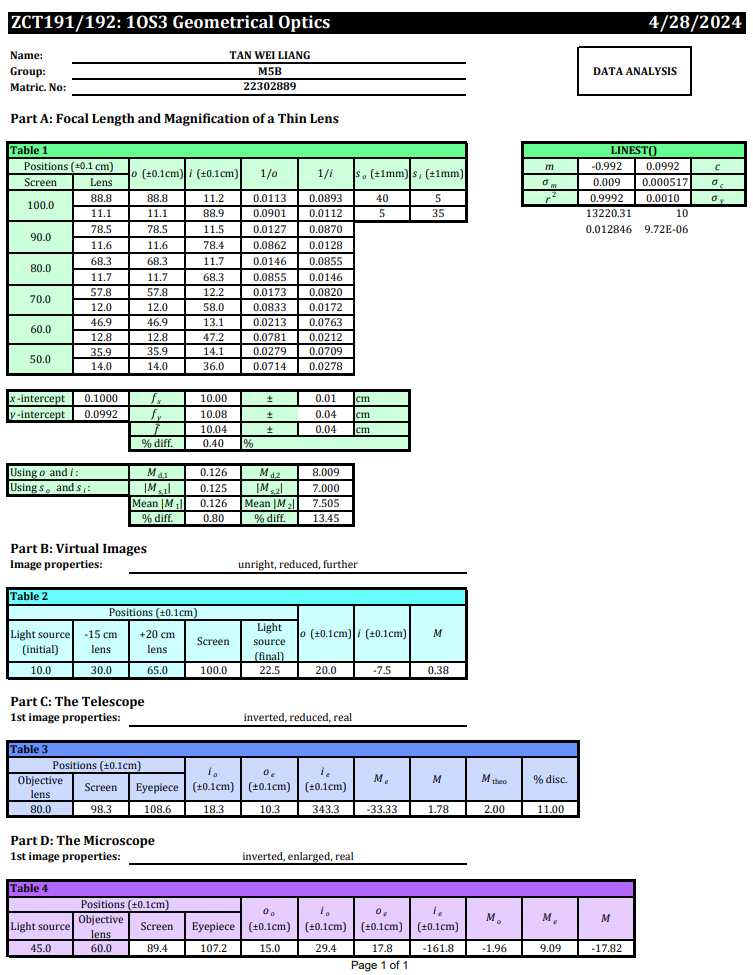
\includegraphics[width=0.89\linewidth]{GO1}
\caption{EXCEL Sheet with experiment data}
\label{6}
\end{figure}
%Part A Calculation
%%%%%
\newpage
\subsection*{Part A Calculation}
To find $x$ intercept, $(\frac{1}{o})_{\text{intercept}}$:\\
~\\
Since $\frac{1}{i} = m\left(\frac{1}{o}\right) + c$, and $(\frac{1}{o})_{\text{intercept}}$ exists when $\frac{1}{i} = 0$,\\
Thus,
\[
(\frac{1}{o})_{\text{intercept}} = -\frac{c}{m} = -\frac{0.0992}{-0.992} = 0.1000\, \text{cm}^{-1}
\]
~\\
The standard error of $x$ intercept:
~\\
\[
\\
\frac{\sigma(\frac{1}{o})_{\text{intercept}}}{(\frac{1}{o})_{\text{intercept}}} = \sqrt{\left(\frac{\sigma c}{c}\right)^2 + \left(\frac{\sigma m}{m}\right)^2}
\]
\[
\sigma(\frac{1}{o})_{\text{intercept}}= 0.1000\sqrt{\left(\frac{0.0005}{0.0992}\right)^2 + \left(\frac{0.009}{-0.992}\right)^2}
\]
\[
\sigma(\frac{1}{o})_{\text{intercept}} \approx 1.0378 \times 10^{-4}
\]
\[
\sigma(\frac{1}{o})_{\text{intercept}} = 0.0001 \,\text{cm}^{-1}
\]
~\\
Therefore, the $x$ intercept of the graph $(0.1000 \pm 0.0001)\, \text{cm}^{-1}$.\\
~\\
To find $f_x$ and $f_y$:\\
~\\
From the equation, $\frac{1}{f} = \frac{1}{o} + \frac{1}{i}$\\
~\\
$\frac{1}{o}$ intercept only exists when $\frac{1}{i}$=0,\\
~\\
\[
\frac{1}{f_x}=(\frac{1}{o})_{intercept}
\]
%%%
To find the $x$-intercept, $f_x$:
\[ f_x = \frac{1}{(\frac{1}{o})_{\text{intercept}}} = \frac{1}{0.1000} = 10.00\,\text{cm} \]
~\\
To find the standard error of $f_x$,
\[ \frac{\sigma_{f_x}}{f_x} = \sqrt{\left( \frac{\sigma(\frac{1}{o})_{\text{intercept}}}{(\frac{1}{o})_{\text{intercept}}} \right)^2} \]
\[ \sigma_{f_x} = 10.00\sqrt{\left( \frac{1.0378 \times 10^{-4}}{0.1000} \right)^2} \]
\[ \sigma_{f_x} \approx 0.0104\, \text{cm} \]
\[ \sigma_{f_x} =0.01\, \text{cm} \]
\\
Therefore, $f_x = (10.00 \pm 0.01)\, \text{cm}$.\\
\\
Likewise, $\frac{1}{i}$ intercept only exists when $\frac{1}{o} = 0$,\\

\[ \frac{1}{f_y} = (\frac{1}{i})_{\text{intercept}} \]

\[ f_y = \frac{1}{(\frac{1}{i})_{\text{intercept}}} = \frac{1}{0.0992} \approx 10.081\, \text{cm} \]

\[ f_y = 10.08\, \text{cm} \]
~\\
To find the standard error of $f_y$,
\[ \frac{\sigma_{f_y}}{f_y} = \sqrt{\left( \frac{\sigma(\frac{1}{i})_{\text{intercept}}}{(\frac{1}{i})_{\text{intercept}}} \right)^2} \]
\[ \sigma_{f_y}= 10.08\sqrt{\left( \frac{0.0005}{0.0992} \right)^2} \]
\[ \sigma_{f_y}\approx 0.0408\, \text{cm} \]
\[ \sigma_{f_y} = 0.04\, \text{cm} \]
~\\
Therefore, $f_y = (10.11 \pm 0.04)\, \text{cm}$.
~\\
To find $\bar{f}$:
\[ \bar{f} = \frac{f_x + f_y}{2} = \frac{10.00 + 10.08}{2} = 10.04\,\text{cm} \]
~\\
To obtain the standard error of $\bar{f}$:
\[ \delta \bar{f} = \sqrt{(\delta f_x)^2 + (\delta f_y)^2} \]
\[ \delta \bar{f} = \sqrt{(0.01)^2 + (0.04)^2} \]
\[ \delta \bar{f} \approx  0.0412 \]
\[ \delta \bar{f} = 0.04 \, \text{cm} \]\\
\\
Therefore, $\bar{f} = (10.04 \pm 0.04)\, \text{cm}$.\\
\\
Percentage difference is calculated by
\[ \text{Percentage difference} = \frac{2|\bar{f} - f|}{|\bar{f} + f|} \times 100\% \]
\[ \text{Percentage difference} = \frac{2|10.04-10|}{10.04+10} \times 100\% \]
\[ \text{Percentage difference} \approx 0.3992\% \]
\[ \text{Percentage difference} =0.40\,\% \]
\\
Percentage discrepancy of $\bar{f}$ and $f_{\text{theo}}$
\[ \text{Percentage discrepancy} = \frac{|\text{experimental value} - \text{theoretical value}|}{\text{theoretical value}} \times 100\% \]
\[ \text{Percentage discrepancy} = \frac{|10.04-10.00|}{10.00} \times 100\% \]
\[ \text{Percentage discrepancy} = 0.40\,\% \]\\
\\
To find the magnification by using object and image distance, \( M_d \):
\[ M_d = -\frac{i}{o} \]
~\\
The magnification of the first image is,
\[ M_{d,1} = -\frac{11.2}{88.8} = -0.126 \]
~\\
The magnification of the second image is,
\[ M_{d,2} = -\frac{88.9}{11.1} = -8.009 \]
~\\
To find the magnification by using object and image size, \( |M_s| \):
\[ |M_s| = \frac{|s_i|}{|s_o|} \]
~\\
The magnification of the first image is,
\[ |M_{s,1}| = \frac{5}{40} = 0.125 \]
~\\
The magnification of the second image is,
\[ |M_{s,2}| = \frac{35}{5} = 7.000 \]
~\\
To find the mean of the magnification:
\[ |M| = \frac{|M_d| + |M_s|}{2} \]
~\\
The mean of the first image is,
\[ |M_1| = \frac{|M_{d,1}| + |M_{s,1}|}{2} = \frac{|-0.126| + |0.125|}{2} = 0.126 \]
~\\
The mean of the second image is,
\[ |M_2| = \frac{|M_{d,2}| + |M_{s,2}|}{2} = \frac{|-8.009| + |7.000|}{2} = 7.505 \]
~\\
Percentage difference of \( |M_1| \) is calculated by
\[ \text{Percentage difference} = \frac{2||M_{d,1}|-|M_{s,1}||}{||M_{d,1}|+|M_{s,1}||} \times 100\% \]
\[ = \frac{2||-0.126| -| 0.125||}{||-0.126|+|0.125||} \times 100\% = 0.80\,\% \]
~\\
Percentage difference of \( |M_2| \) is calculated by
\[ \text{Percentage difference} = \frac{2||M_{d,2}|-|M_{s,2}||}{||M_{d,2}|+|M_{s,2}||} \times 100\% \]
\[ = \frac{2||-8.009| - |7.000||}{||-8.009|+|7.000||} \times 100\% = 13.45\,\% \]
%%%%%
\newpage
\subsection*{Part B Calculation}
Experimentally, $i$ = -7.5 cm, \\
\begin{align*}
\text{Object distance, } o &= 30.0 - 10.0 \\
o &= 20.0 \, \text{cm} \\
\text{Image distance, } i &= 22.5 - 30.0 \\
i &= -7.5 \, \text{cm} \\
\end{align*}
Theoretically, $i_{theo}$ = -8.57 cm, \\
\begin{align*}
\frac{1}{f_{concave}} &= \frac{1}{o} + \frac{1}{i_{theo}}\\
\frac{1}{-15.0} &= \frac{1}{20.0} + \frac{1}{i_{theo}}\\
i_{theo} &= -8.57 cm\\
\end{align*}
Percentage discrepancy of $i$,
\begin{align*}
\text{Discrepancy of } i &= \frac{|\text{experimental value} - \text{theoretical value}|}{|\text{theoretical value}|} \times 100\%\\
&= \frac{|-7.5 -(-8.57)|}{|-8.57|} \times 100\%\\
&= 12.49 \%
\end{align*}
For magnification part,\\
\\
Experimentally,
\begin{align*}
M &= \frac{-i}{o} = \frac{-(-7.5)}{20.00} = 0.375
\end{align*}\\
due to the positive value of magnification indicated that the virtual image is upright.\\
\\
Theoretically,
\begin{align*}
M_{theo} &= \frac{-i}{o} = \frac{-(-8.57)}{20.00}  \approx 0.4285 \\
M_{theo} &= 0.429
\end{align*}\\
Percentage discrepancy of $M$,
\begin{equation*}
\text{Percentage discrepancy of } M = \frac{|0.375 - 0.429|}{0.429} \times 100\% = 12.59\%
\end{equation*}
%%%%%
\newpage
\subsection*{Part C Calculation}
To find $ i_e$,\\
\\
\begin{equation*}
\frac{1}{f} = \frac{1}{o_e} + \frac{1}{i_e}
\end{equation*}
\\
\text{Given:}
\begin{equation*}
f = 10 \, \text{cm} \quad \text{and} \quad o_e = 10.3 \, \text{cm}
\end{equation*}\\
\\
\text{Solve for } $i_e$,
\begin{align*}
i_e &= \frac{1}{\frac{1}{f} - \frac{1}{o_e}} = \frac{1}{\frac{1}{10} - \frac{1}{10.3}} \approx 343.333\\
 i_e &= 343.3 \, \text{cm}
\end{align*}\\
\\
Magnification ($M_e$),
\begin{align*}
M_e = -\frac{i_e}{o_e}
\end{align*}\\
\\
\text{Calculated,}
\begin{align*}
M_e &= \frac{-(343.3)}{10.3} \approx -33.33009 \\
M_e &= -33.33
\end{align*}\\
\\
\text{Using the objective lens ($M$),}
\begin{equation*}
M = \frac{i_o}{o_o}
\end{equation*}\\
\\
\text{Given:}
\begin{equation*}
i_o = 18.3 \, \text{cm} \quad \text{and} \quad o_e = 10.3 \, \text{cm}
\end{equation*}\\
\\
\text{Solve for } $M$,
\begin{align*}
M &= \frac{18.3}{10.3} \approx 1.7767\\
M &= 1.78
\end{align*}\\
\\
\text{Solve for } $M_{theo}$,
\begin{align*}
M_{theo} &=\frac{f_o}{f_e}\\
 &= \frac{20}{10}\\
 &= 2.00
\end{align*}\\
\\
Percentage discrepancy of $M$ and $M_{theo}$,
\begin{align*}
\text{Discrepancy} &= \frac{|\text{experimental value} - \text{theoretical value}|}{\text{theoretical value}} \times 100\%\\
&= \frac{|1.78- 2.00|}{2.00} \times 100\%\\
&= 11.00\%
\end{align*}
%%%%%
\newpage
\subsection*{Part D Calculation}
To find \( i_e \):

\begin{equation*}
\frac{1}{f} = \frac{1}{o_e} + \frac{1}{i_e}
\end{equation*}
\\
\text{Given:}
\begin{equation*}
f = 20 \, \text{cm} \quad \text{and} \quad o_e = 17.8 \, \text{cm}
\end{equation*}
\\
\text{Solve for} \( i_e \):
\begin{align*}
i_e &= \frac{1}{\frac{1}{f} - \frac{1}{o_e}} = \frac{1}{\frac{1}{20} - \frac{1}{17.8}} \approx -161.818\\
i_e &= -161.82 \, \text{cm}
\end{align*}
\\
Magnification (\( M_o \) and \( M_e \)):
\\
\begin{align*}
M_o &= -\frac{i_o}{o_o} \\
M_e &= -\frac{i_e}{o_e}
\end{align*}
\\
\text{Calculated:}
\begin{align*}
M_o &= -\frac{29.4}{15.0} = -1.96 \\
M_e &= -\frac{ -161.82}{17.8} \approx 9.091\\
M_e &= 9.09
\end{align*}
\\
Total magnification (\( M \)):
\begin{align*}
M &= M_e \cdot M_o\\
M &= (9.09) \cdot (-1.96) \approx -17.816\\
M &= -17.82
\end{align*}
\end{document}    